\begin{flushright} {\tiny {\color{gray} benchmark\_scbe08.tex}} \end{flushright}
%~~~~~~~~~~~~~~~~~~~~~~~~~~~~~~~~~~~~~~~~~~~~~~~~~~~~~~~~~~~~~~~~~~~~~~~~~~~~~~~~~~~~~~~~~~~~~~~~~~

\vspace{0.5cm}
\begin{flushright}
Data pertaining to this section are to be found at:
\url{https://github.com/cedrict/fieldstone/tree/master/images/benchmark_scbe08}
\end{flushright}
\vspace{0.5cm}

The setup is as follows :

\begin{center}
\includegraphics[width=7cm]{images/benchmark_scbe08/setup}\\
{\captionfont Taken from Schmeling \etal (2008) \cite{scbe08}.}
\end{center}

Materials are linear viscous, initial geometry is simple, 
boundary conditions are simple. On paper it sounds like a 
good idea. See \stone 67 for a discussion on why this 
setup was doomed from the beginning as a benchmark.  

Experiments have been conducted by a handful of codes, 
investigating the effect of averaging and mesh resolution:

\begin{center}
\includegraphics[height=6cm]{images/benchmark_scbe08/scbe08_2}
\includegraphics[height=6cm]{images/benchmark_scbe08/scbe08_1}
\includegraphics[height=6cm]{images/benchmark_scbe08/scbe08_3}\\
{\captionfont Taken from Schmeling \etal (2008) \cite{scbe08}.
Left: case 1 model (here FDCON-4 is shown). Streamlines are also shown.
Middle: Shapes of different case 1 models at similar stages: FDCON: 40 Myears,
I2ELVIS: 34.7 Myears, CITCOM: 38.1 Myears. Viscosity averaging: geometric mean
in all cases.
Right: Comparison of the shapes of the slabs for different viscosity averaging meth-
ods using I2VIS. Note that the snapshots are taken at different times (59.6, 24.4,
37.8 Myears from top to bottom), so that the slab tips have reached comparable
levels.}
\end{center}

\begin{center}
\includegraphics[height=5cm]{images/benchmark_scbe08/scbe08_4}
\includegraphics[height=5cm]{images/benchmark_scbe08/gltf18}\\
{\captionfont 
Temporal behaviour of case 1 modelled by different codes with highest resolutions each. 
Each curve shows the position of the deepest part of the slab (slab tip) as
a function of time below the initial surface of the lithosphere.
Left: taken from Schmeling \etal (2008) \cite{scbe08}; 
Right:taken from Glerum \etal (2018) \cite{gltf18}.}
\end{center}

\begin{center}
\includegraphics[height=5cm]{images/benchmark_scbe08/scbe08/slab_tip_depth.pdf}\\
{\captionfont Data curtesy of Prof. H. Schmeling.}
\end{center}



